\documentclass[11pt]{article}
\usepackage[margin=1in]{geometry}
\usepackage{amsmath,amssymb,amsthm}
\usepackage{booktabs,enumitem,graphicx,xcolor,listings}
\usepackage{xurl}
\usepackage[colorlinks=true,linkcolor=blue!50!black,citecolor=green!35!black,urlcolor=blue!50!black]{hyperref}
\usepackage[nameinlink]{cleveref}
\lstset{basicstyle=\ttfamily\footnotesize,columns=fullflexible,frame=single,framerule=0.3pt,rulecolor=\color{gray!60}}
\theoremstyle{definition}\newtheorem{definition}{Definition}

\title{The Posterior Coherence Engine:\\ Separating Uncertainty from Incoherence}
\author{V.~K. Awasthi}
\date{October 2026}

\begin{document}
\maketitle

\begin{abstract}
When several sources report on the same question, averaging their reports answers one question: how uncertain is the answer? It
cannot answer a second: do the reports admit one coherent model at all? The Posterior Coherence Engine keeps these apart. For a set
of local reports it returns (i) the three-level split of predictive uncertainty into disagreement between groups, disagreement within
groups and irreducible noise; (ii) a coherence status, either coherent and unique, coherent but not unique (with the width of the set of
global laws), or incoherent (with a finite certificate and a consistency radius); and (iii) the Beck--Chevalley defect of a pooling
rule, which says when pooling is exact. A decision layer answers, abstains, or flags. On synthetic worlds with known truth, the averaged
answers carry no information about incoherence, while the consistency radius detects it with AUROC rising from $0.58$ to $0.92$ as data
per context grow. In a pre-registered test on 2358 items answered by four runs of two model families, keeping where disagreement sits
improves the prediction of whether the pooled answer is correct by $0.0175$ bits per item ($95\%$ interval $[0.0107,0.0241]$), with
the gain concentrated in the two tasks with strong version drift. The incoherence detector cannot be tested on these data, because each
item's answers are observed jointly; we say what data would test it.
\end{abstract}

\section{What the engine reports}
The inputs are local reports: probability tables on \emph{windows} (sets of variables observed together), and, where available,
posteriors from sources arranged in groups. The engine returns three things.

\paragraph{1. Uncertainty about the answer.} For groups $g$ with weights $w_g$ and member posteriors $q$, the chain rule along
(group, member) gives exactly
\[
H(\rho)\;=\;\underbrace{I(X;\text{group})}_{\text{between}}\;+\;\underbrace{I(X;\text{member}\mid\text{group})}_{\text{within}}\;+\;\underbrace{\mathbb E\,H(q)}_{\text{noise}},
\]
where $\rho$ is the overall average. Averaging keeps only $H(\rho)$. This is the martingale structure of the posterior tower
\cite[Thm.~5.3]{Main}.

\paragraph{2. Coherence of the evidence.} Can the window tables be glued into one global law? The engine solves three linear programs.
\begin{itemize}[nosep]
\item The \emph{consistency radius}: the smallest average total-variation adjustment of the window tables that admits a global law.
\item If the radius is $0$: the range of every atom's probability over all global laws. Width $0$ means the global law is unique.
\item If the radius is positive: a \emph{certificate}, found by Farkas duality, a functional on window cells that is $\ge0$ on every
  deterministic assignment (hence on every global law) and negative on the data. For three binary claims seen in pairs it is a cycle
  (Bell-type) inequality such as $\Phi\le2$ \cite[Prop.~16.1]{Main}.
\end{itemize}
Two overlapping windows always glue; failure needs a cycle in the cover \cite[Prop.~16.3]{Main}.

\paragraph{3. Validity of pooling.} For two windows meeting in $M$, pooling through $M$ (the Markov glue) is exact iff the windows
satisfy Beck--Chevalley, with defect $c$ the largest conditional correlation \cite[Thm.~14.4]{Main}. For a more and a less informed
source, the pooling rules at least as good as the better one form a KL ball of radius $I(X;q_j\mid q_i)$ around the Bayes pool, and every
rule in it errs at most $\sqrt{2I}$ more often (weighted by margin) than the Bayes decision \cite[Thm.~7, Prop.~9]{Pooling}.

\paragraph{Decisions.} \texttt{decide} flags incoherent evidence with its certificate instead of averaging it, flags non-unique
reconstructions whose width exceeds a tolerance, and otherwise answers or abstains by a confidence threshold.

\section{Using it}
\begin{lstlisting}
from pce import Window, coherence, split, decide
import numpy as np
t = np.array([[0.125, 0.375], [0.375, 0.125]])   # each pair agrees w.p. 1/4
dom = {"X0": 2, "X1": 2, "X2": 2}
pairs = [("X0", "X1"), ("X1", "X2"), ("X0", "X2")]
r = coherence(dom, [Window(p, t) for p in pairs])
r.status, r.radius, r.violation    # 'incoherent', 0.083, 0.375
s = split([[(1, [0.9, 0.1]), (1, [0.8, 0.2])],
           [(1, [0.2, 0.8]), (1, [0.3, 0.7])]])
s.between, s.within, s.noise       # 0.282, 0.012, 0.699 bits
decide(s, r).action                # 'flag-incoherent'
\end{lstlisting}
The same evidence, written as a JSON file, runs from the command line:
\begin{lstlisting}
python -m pce.cli examples/three_token.json
\end{lstlisting}

\paragraph{Checks.} \texttt{check\_pce.py} (six checks, all passing) verifies that the engine reproduces the paper's three-token
model (incoherent iff $\varepsilon<\tfrac13$, fibre width $2\min(a,b)$ above), that every certificate is non-negative on all
deterministic assignments and negative on the data (75 incoherent cases among 300 random compatible families), that the split is exact,
that the defect matches $|2\varepsilon-1|/(2\varepsilon)$, that the KL-ball radius matches the companion note, and that the decision
layer acts as specified.

\section{Synthetic demonstrations}
These use worlds with known truth. They debug and illustrate; nothing in the real-data analysis was chosen from them.

\paragraph{Averaging hides conflicts.} Random compatible pair tables on a triangle of binary claims, about a quarter of which admit no
global law, are observed with $n$ samples per pair. The confidence of the averaged per-claim answers does not distinguish the two
classes (AUROC between $0.40$ and $0.52$); the consistency radius does, with AUROC $0.58$, $0.75$, $0.84$ and $0.92$ at $n=25$, $100$,
$400$ and $1600$ (\cref{fig:engine}a). Many random incoherent families are only barely incoherent, which is why small samples struggle.

\paragraph{Non-unique reconstruction.} When only the chain $(X_0,X_1)$, $(X_1,X_2)$ is observed, the engine reports the interval of
$P(X_0=X_2)$ over all global laws. Over 200 random worlds the interval always contains the truth; the single Markov-glue reconstruction
never equals it, with median error $0.09$ and maximum $0.36$.

\paragraph{Where disagreement sits.} Items are answered by four runs in two families. In a world with family-specific blind spots,
adding the between-family term to $(v,H)$ improves out-of-fold log loss by $0.036$ bits ($[0.017,0.052]$) and AUROC from $0.78$ to
$0.81$. In a null world with exchangeable runs it changes nothing ($-0.0004$ bits, $[-0.002,0.001]$). So the test can fail, and does
when there is nothing to find.

\section{A pre-registered real-data test}
\paragraph{Design.} The plan was frozen before any outcome was computed (\texttt{study4/PREREG\_engine.md}, SHA-256 beginning
\texttt{5c6543bf}). Data: the LLM-drift answers of GPT-4 (March, June) and GPT-3.5 (March, June) on five tasks \cite{ChenZaharia2024},
2358 items with all four answers and a reference. The pooled answer is the plurality (ties to GPT-4 June). The question is whether the
pooled answer is correct. The averaging baseline uses only the pooled vote distribution: vote share $v$ and entropy $H$. The engine adds
the between-family term $B$. Both are logistic models fitted within task, scored by five-fold out-of-fold log loss.

\begin{figure}[t]\centering
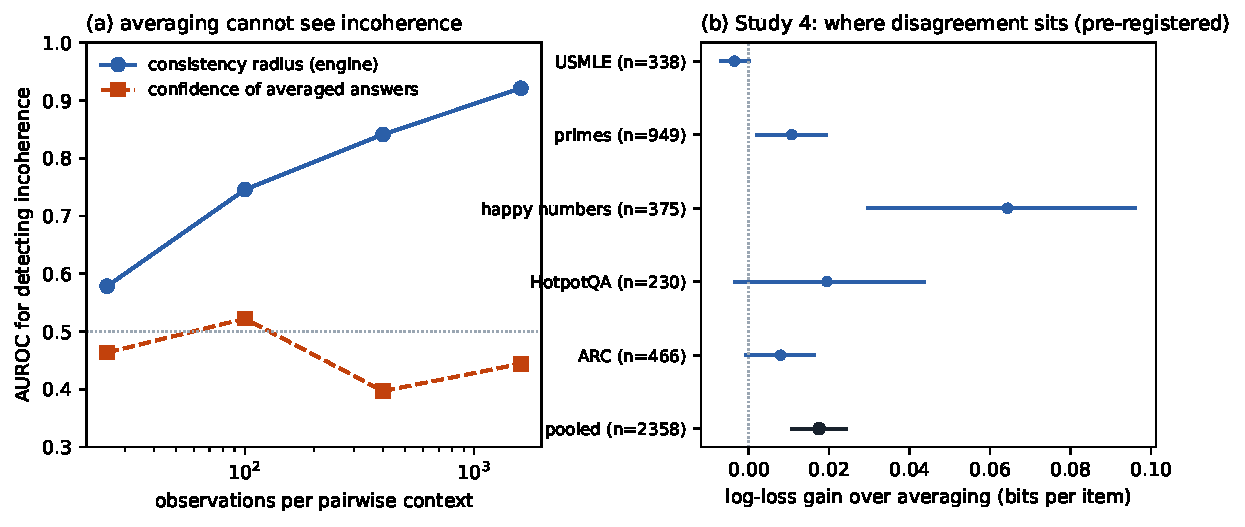
\includegraphics[width=\linewidth]{fig_engine}
\caption{(a) Detecting incoherent evidence on synthetic triangles: the engine's consistency radius against the confidence of averaged
answers. (b) Study 4: gain in out-of-fold log loss from adding the between-family term, per task and pooled, with $95\%$ bootstrap
intervals. Pre-registered.}
\label{fig:engine}
\end{figure}

\begin{table}[t]\centering\small
\caption{Study 4 (pre-registered). $\Delta$ = log-loss gain of the engine over averaging, bits per item; one-sided bootstrap $p$,
Holm-adjusted; AUROC of out-of-fold probabilities.}
\label{tab:s4}
\begin{tabular}{lrcccc}\toprule
task & $n$ & accuracy & $\Delta$ [95\% interval] & $p_{\mathrm{Holm}}$ & AUROC: averaging $\to$ engine\\\midrule
USMLE & 338 & 0.861 & $-0.0035$ [$-0.0067$, 0.0000] & 0.974 & 0.643 $\to$ 0.625\\
primes & 949 & 0.542 & 0.0107 [0.0020, 0.0191] & 0.016 & 0.873 $\to$ 0.874\\
happy numbers & 375 & 0.635 & 0.0644 [0.0298, 0.0961] & 0.005 & 0.690 $\to$ 0.842\\
HotpotQA & 230 & 0.600 & 0.0195 [$-0.0034$, 0.0436] & 0.100 & 0.689 $\to$ 0.707\\
ARC & 466 & 0.273 & 0.0080 [$-0.0005$, 0.0162] & 0.091 & 0.788 $\to$ 0.790\\\midrule
pooled & 2358 & & \textbf{0.0175 [0.0107, 0.0241]} & & 0.870 $\to$ 0.875\\\bottomrule
\end{tabular}
\end{table}

\paragraph{Result.} The pre-registered hypothesis is supported: keeping where disagreement sits improves the decision by $0.0175$ bits
per item, with interval $[0.0107,0.0241]$ (\cref{tab:s4}). The gain is significant after Holm correction in two tasks, primes and happy
numbers, positive but not significant in HotpotQA and ARC, and slightly negative in USMLE.

\paragraph{Exploratory reading.} In primes, 475 of 949 items split two against two \emph{within} each family (the March and June
versions of each model disagree), and the pooled answer is right on only $19\%$ of them; in happy numbers the same pattern has accuracy
$4\%$ (48 items). Splits \emph{along} family lines are rare and much more often right. At equal total entropy, disagreement within a
family over time predicts error more strongly than disagreement between families; the fitted coefficient on $B$ is positive in primes,
happy numbers and ARC. The gain is therefore concentrated where model versions drifted, which Chen et al.\ documented for exactly these
tasks. It is a real effect of the information the engine keeps, but it should not be read as a general property of all tasks.

\section{What is not yet tested}
\begin{itemize}[nosep]
\item \emph{Incoherence on real data.} Each item's answers in Study 4 are observed jointly, and jointly observed tables always admit a
  global law, so the engine's coherence status is uninformative there. A real test needs evidence gathered in separate contexts, for
  example asking a model about pairs of related claims in separate prompts. The pairwise-elicitation kit of the main paper
  (\texttt{halluc\_study/kit\_pairwise\_cycles.py}) collects such data; the engine scores it directly.
\item \emph{Decisions beyond correctness prediction.} Study 4 measures how well the engine's features predict whether the pooled answer
  is right. Whether flagging and abstaining by the engine improves a downstream task is the next experiment, and should be
  pre-registered in the same way.
\item \emph{Statistical calibration of the radius.} The radius is a point estimate; a bootstrap or permutation calibration for finite
  samples, as done for the Beck--Chevalley test in the main paper, would turn it into a test with known error rates.
\end{itemize}

\section*{Code}
The package \texttt{pce}, the checks, the demonstrations and Study 4 are in the \texttt{engine} folder of
\url{https://github.com/vkawasth/Trainingless-Transformer-NoGradientDescent/tree/main/papers}.

\begin{thebibliography}{9}
\bibitem{Main} V.~K. Awasthi, Shadows, fibres and secants of the posterior tower. Technical report, October 2026.
\bibitem{Pooling} V.~K. Awasthi, Pooling informed agents: Blackwell order, reconciliation and the KL ball. Companion note, October 2026.
\bibitem{ChenZaharia2024} L.~Chen, M.~Zaharia and J.~Zou, How is ChatGPT's behavior changing over time? \emph{Harvard Data Science
  Review} \textbf{6} (2024), no.~2; arXiv:2307.09009. Data: \url{https://github.com/lchen001/LLMDrift}.
\end{thebibliography}
\end{document}
